\section{Model fit coefficients} \slabel{fit}
\begin{table*}
\setlength{\tabcolsep}{12pt}
\centering
\pgfplotstabletypeset[
  col sep=space,
  columns/Gr/.style={sci,sci 10e,precision=1},
  columns/Ra/.style={sci,sci 10e,precision=1},
  columns/Sc/.style={column type/.add={}{|}},
%every first column/.style={
%column type/.add={|}{}
%},
%every last column/.style={
%column type/.add={}{|}
%},
  columns/$C_1$/.style={fixed,zerofill,precision=2},
  columns/$C_2$/.style={fixed,zerofill,precision=1,dec sep align},
  columns/$C_3$/.style={fixed,zerofill,precision=2},
  columns/$C_7$/.style={fixed,zerofill,precision=2},
  columns/$C_5$/.style={fixed,zerofill,precision=2, column type/.add={}{|}},
  columns/$E_d$/.style={
        column type=r,
        dec sep align,
        preproc/expr={100*##1},
        postproc cell content/.append code={
            \ifnum1=\pgfplotstablepartno
                \pgfkeysalso{@cell content/.add={}{\%}}%
            \fi
        },
        fixed,
        fixed zerofill,
  },
  columns/$E_m$/.style={
        column type=r,
        dec sep align,
        preproc/expr={100*##1},
        postproc cell content/.append code={
            \ifnum1=\pgfplotstablepartno
                \pgfkeysalso{@cell content/.add={}{\%}}%
            \fi
        },
        fixed,
        fixed zerofill,
  },
  every head row/.style={
        before row=\toprule,after row=\midrule},
  every row no 1/.style={after row=\midrule},
  every row no 4/.style={after row=\midrule},
  every row no 8/.style={after row=\midrule},
  every row no 13/.style={after row=\midrule},
  every row no 17/.style={after row=\midrule},
  every last row/.style={
        after row=\bottomrule},
]{tbl/coef.dat}
\caption{ 
Simulation conditions, fit coefficients, and relative errors. 
}
\end{table*}

\subsection{Fitting}

\begin{figure}
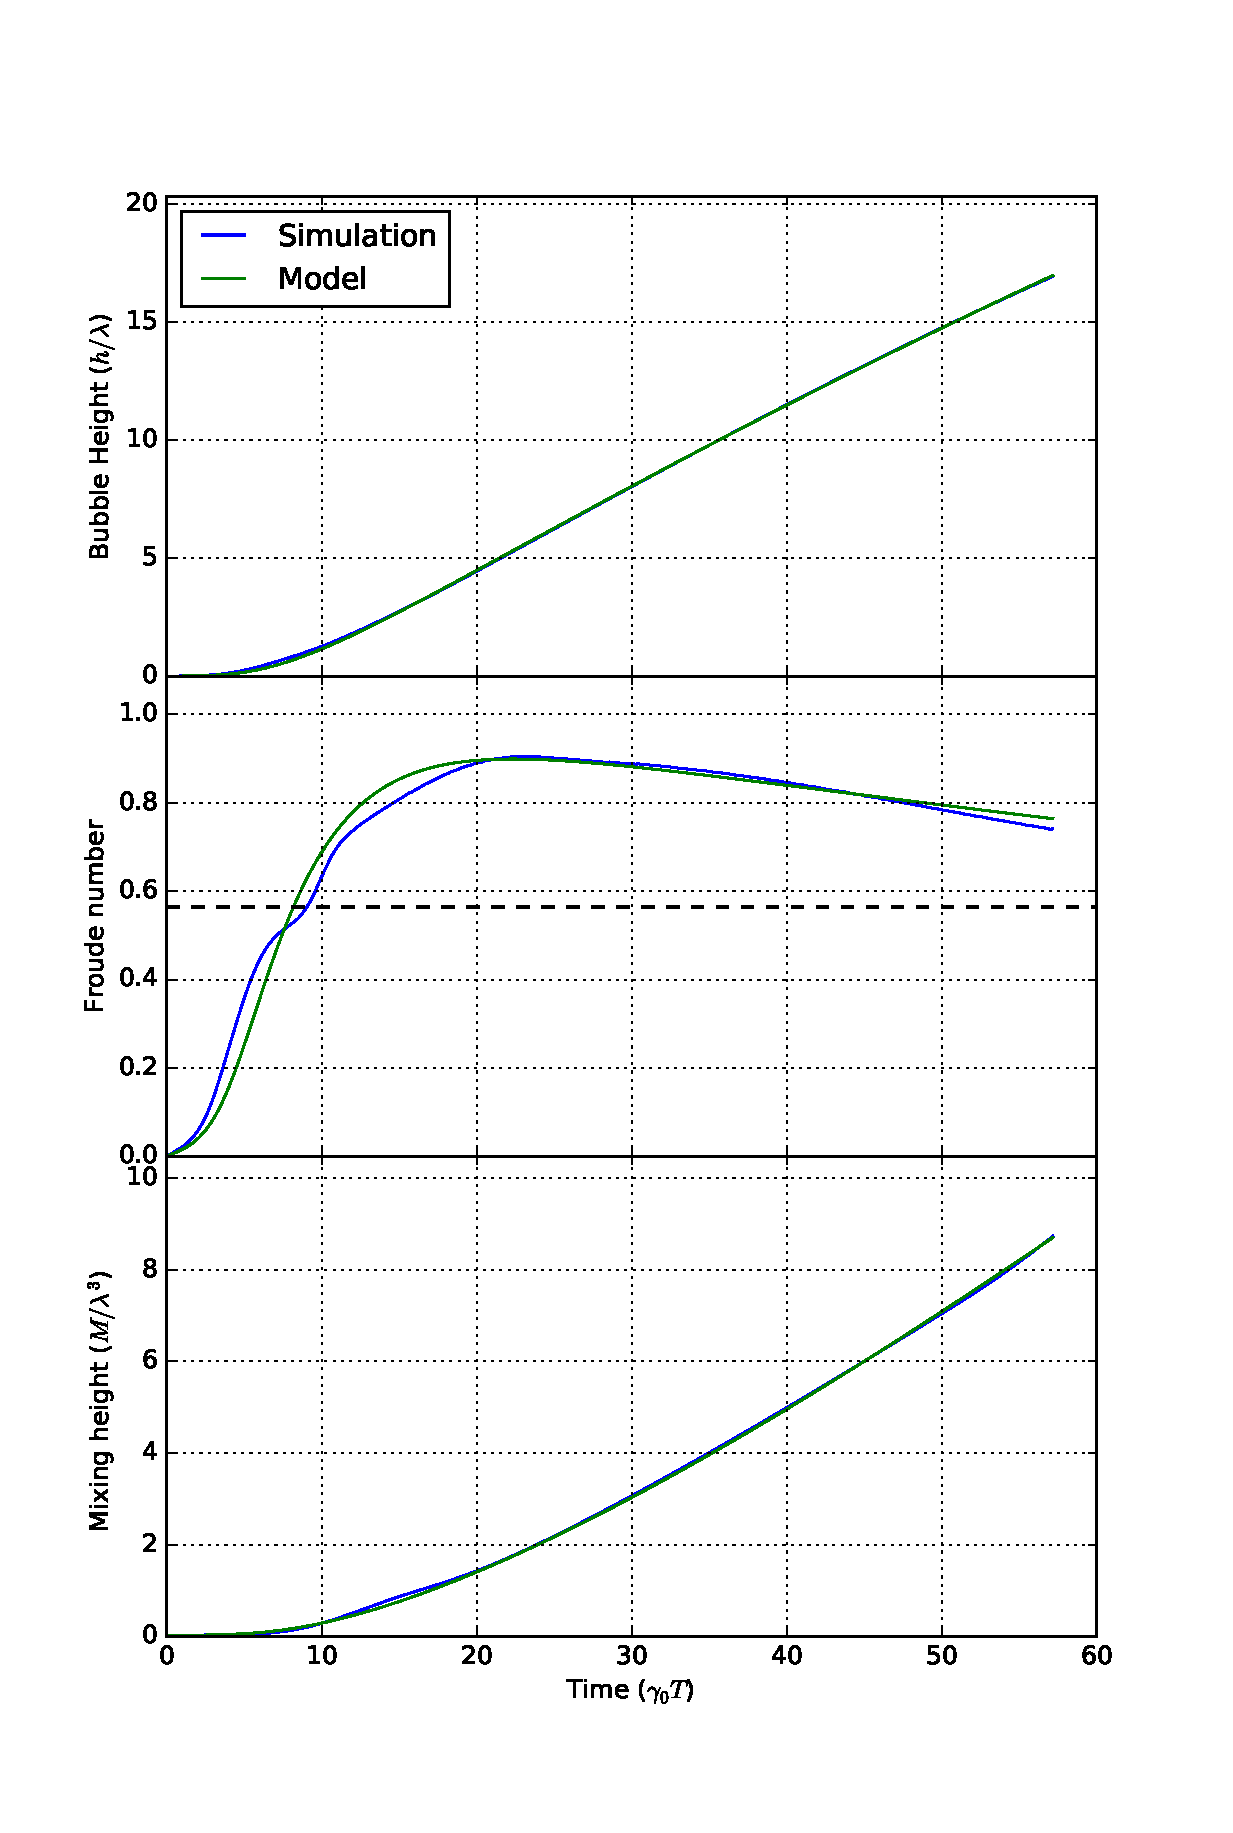
\includegraphics[height=\textheight]{figs/H-8-1}
\caption{ \flabel{example_fit}
  Example fit of the bubble height, top, and mixed volume, bottom, at $\text{Ra} = $ and $\text{Sc} = 8$.
  The dashed line is center plot is the stagnation velocity from potential flow models.
  The Froude number, which is a non-dimensional velocity, is not directly fit but shows agreement between the model and simulation.
}
\end{figure}

The mixing model defines the quantity of mixed fluid, $m(t)$, as an analytic function:
\begin{equation}
\left\{H(t), \delta(0), \lambda, D, C_5\right\} \rightarrow m(t),
\end{equation}
where $H(t)$ is the bubble height, 
$\delta(0)$ is the initial interface thickness,
$\lambda$ is the wavelength,
$D$ is the diffusivity, and 
$C_5$ is a mixing coefficient.
The values of $H(t)$, $\delta(0)$, $\lambda$, and $D$ are taken from the numerical experiments, allowing for the definition of an mixing error:
\begin{equation}
E_m = \left|\left|m\left[C_5\right] - M(t) \right| \right|_2,
\end{equation}
where $M(t)$ is the reference value from the numerical experiments.
To compute $C_5$, the error is minimized under the constraint $C_5 > 0$.
The fitting problem is non-linear but 1D dimensional, so it can be solved with a sequential least squares minimizer, which finds local minima, wrapped with a basin hopping scheme, which samples across the local minima.

The dynamics model defines the bubble height, $h(t)$, as the solution to an ordinary differential equation.
The dynamics model is integrated using the variable-coefficient ordinary differential equation (VODE) solver for stiff systems, creating a map from the dynamics coefficients to the height:
\begin{equation}
\left\{h(0), \delta(0), \lambda, \nu, D, C\right\} \rightarrow h(t),
\end{equation}
where $h(0)$ is the initial bubble height,
$\delta(0)$ is the initial interface thickness,
$\lambda$ is the wavelength,
$\nu$ is the kinematic viscosity,
$D$ is the diffusivity, and
$C$ are the model coefficients.
$\delta(0)$, $\lambda$, $\nu$, and $D$ are taken from the simulation while $C_5$ is taken from independently fitting the mixing model, allowing for the definition of a dynamics error:
\begin{equation}
E_d = \left| \left| h\left[C_1, C_2, C_3, C_7\right] - H(t)\right| \right|_2,
\end{equation}
where $H(t)$ is the reference value from the numerical experiments.
The non-linear global minimization problem is solved with the covariance matrix adaptation evolution strategy (CMA-ES).
CMA-ES iteratively refines a sample distribution that evolves towards the global optimum.
Computing the model error is very inexpensive compared to the simulations, so we choose a broad initial distribution with a large population size.
The stochastic solution is polished with a sequential least-squares local minimization.

However, the high Rayleigh trajectories are incomplete, in that the data ends when the bubble gets close to the top wall, leading to under-constrained systems.
Therefore, we regularize the fit by adding a term to the model error:
\begin{equation}
R = \beta \left| \left| \frac{C - \bar{C}}{\bar{C}} \right| \right|_2,
\end{equation}
where $\beta$ is the regularization parameter,
$C$ is the vector of model coefficients, and
$\bar{C}$ are the coefficient estimates.
Although the buoyancy-drag model is non-linear, this L2 regularization can be thought of as a Tikhonov regularization~\cite{roths2001generalized} or ridge regression~\cite{marquardt1975ridge}.
The regularization parameter is chosen to be an order smaller than the model error, $\beta = 0.1 E_d$.
The if the regularized dynamic error ends up lower than the unregularized error, the unregularized problem must not have converged to the local minima.
In those cases, the unregularized fit is repeated with the regularized coefficient values as a starting seed.
Then the regularized fit is repeated with the updated definition.
In this way, the two types of fits are iterated until consistency is reached.

The fitting process defines a mapping from the Grashof and Schmidt numbers to the model coefficients and model errors:
\begin{equation}
\left(\text{Gr}, \text{Sc}\right) \rightarrow \left(C_1, C_2, C_3, C_5, C_7, E_m, E_d\right) 
\end{equation}
The rest of this section explores the relationships in this mapping.

\subsection{Scope of the models}

The proposed models aim to describe the mixing and dynamics in rising Rayleigh-Taylor bubbles and falling Rayleigh-Taylor spikes.
The symmetry of the governing equations equates the spike behavior to that of the bubbles, so we will omit spikes from the following discussions.
In highly viscous and diffusive cases, the bubbles may not reach late time highly non-linear dynamics.
For this analysis, a bubble is considered to be covered by the model only if its height exceeds its wavelength before it stops rising.
Experiments which do not meet that condition are discarded.

The bubble grows until mixing dilutes its buoyancy sufficiently for it to stop rising.
After this point, it slowly recedes due to diffusing across the bubble tip.
The model does not account for this diffusive effect, which moves move the center of the interface rather than just broadened it, so bubble trajectories are clipped beyond the point at which the bubble velocity is zero.
The height at that point in the trajectory is maximal and called the \textit{penetration depth}.

The penetration depth increases with Rayleigh number.
For high Rayleigh number cases, the bubble continues to grow until it beings to interact with the top boundary, given the finite computational domain.
Based on previous validation studies~\cite{Hutchinson2016}, we clip the trajectory when the bubble height reaches 75\% of the domain height.
Experiments in which this clipping occurs are incomplete.
Those cases should be re-simulated with a larger computational domain, at greater computational cost, to collect trajectories which reach their penetration depth.

However, there is still information in the incomplete experiments.
In the following sections, incomplete experiments will be marked as such, but the trend in the complete experiments is often seen to continue smoothly into incomplete ones.
Though not definitive, those suggest that the data present in the incomplete experiments is sufficient to constrain the corresponding characterization of the flow.
Conversely, in some cases the behavior in the incomplete experiments departs from that in the complete ones. 
In those cases, it is difficult to differentiate between Rayleigh-dependent behavior and the side-effects of underconstrained fitting.

It should be noted that the computational cost of a complete trajectory goes as $\text{Gr}^4 \text{Ra}^2 \max(1, \text{Sc}^4)$.
The fourth power of the Grashof and Schmidt numbers come from stability constraints: three from the spectral constraint and 1 from the explicit time-stepping constraint.
The square of the Rayleigh number comes from the penetration depth, which both increases the length of the domain and the number of time-steps taken.
For $\text{Sc} \ge 1$, the cost simplifies to $\text{Ra}^6$.
For the runs in this study, the cheapest incomplete trajectories will cost $64\times$ more than most expensive completed ones.
The most expensive incomplete trajectory, at $\text{Ra} \approx 1.4\times 10^6$, will cost over $10^9\times$ more than cheapest completed one.

\subsection{Accuracy of the models}

\begin{figure*}
\begin{subfigure}[b]{0.5\textwidth}
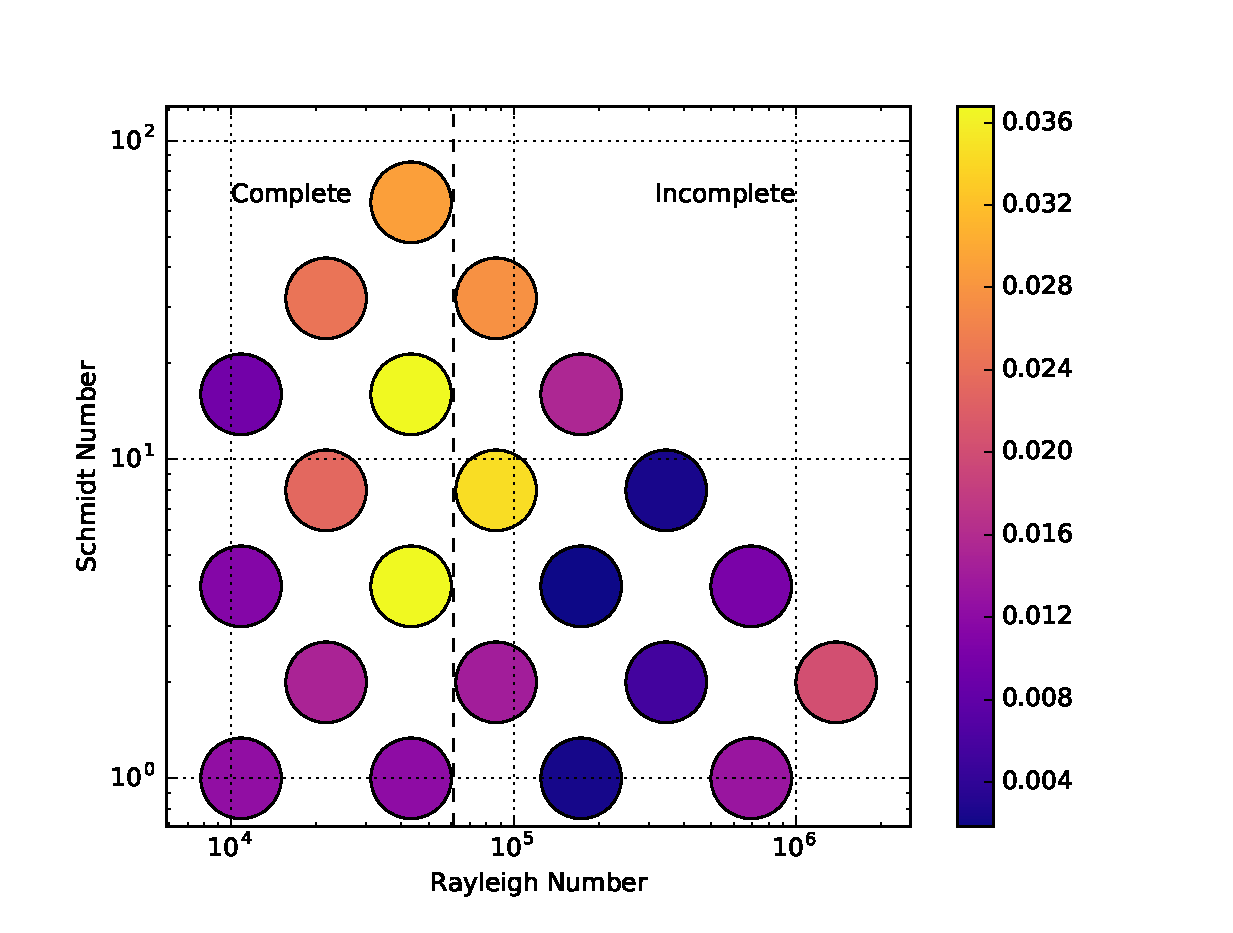
\includegraphics[width=\textwidth]{figs/MixingError-vs-Rayleigh-Schmidt}
\caption{Relative mixing error, $E_m/\text{max}[M(t)]$}
\end{subfigure}
\begin{subfigure}[b]{0.5\textwidth}
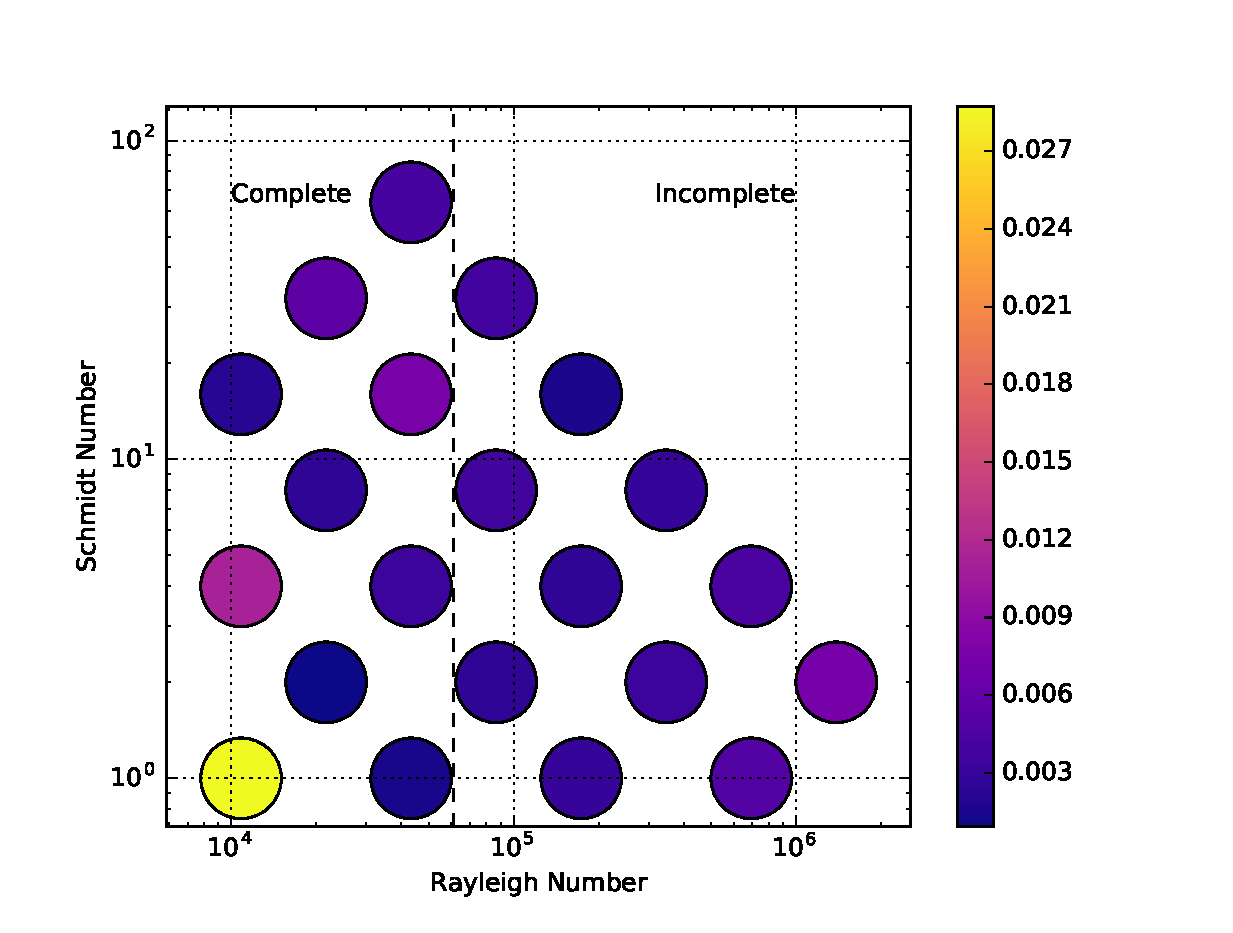
\includegraphics[width=\textwidth]{figs/DynamicsError-vs-Rayleigh-Schmidt}
\caption{Relative dynamics error, $E_d/\text{max}[H(t)]$}
\end{subfigure}
\caption{ \flabel{errVsParam}
  Relative model errors versus Rayleigh and Schmidt numbers.
  Experiments on the left side of the dashed line completed when the bubble stopped rising.
  Experiments on the right side of the dashed line are incomplete, having approached the vertical boundaries of the simulated domain.
}
\end{figure*}

The accuracy is characterized by the mixing and dynamics model errors relative to the maximum mix volume and bubble height, respectively.
The relative model errors are plotted versus the Rayleigh and Schmidt numbers in \fref{errVsParam}.
In both models, the nominal error is less than 5\%, but the two errors have differing structures.

The relative mixing error is about 3\% for the complete experiments, with generally greater relative error at greater Rayleigh and Schmidt numbers.
Among the incomplete experiments, relative error decreases with Rayleigh number before increasing again.
This is likely due to the incompleteness; the greater error above $\text{Ra} = 10^6$ suggests that the overall trend is increasing.
Overall, the relationship between the accuracy of the mixing model the Rayleigh and Schmidt numbers is incomplete.

The relative dynamics error is about 1\%, with the exception of the unit Schmidt $\text{Ra} \approx 10^4$ case.
The mixing error for the outlying case is typical, so the error cannot be attributed to the treatment of mixing.
This case will be considered more in the following sections.
Outliers aside, the relative error decreases with Schmidt number and Rayleigh number, both for complete and incomplete trajectories.
This indicates the dynamics model is most accurate, at least relative to the mixing height, when there is less mixing and drag.
Another factor is re-acceleration, which adds some relatively constant error that is amortized more when the penetration depth is greater.


\begin{comment}
The model proposed in \sref{model} assumes the bubble is a coherent structure with a single velocity.
If the Grashof number is high, then the bubble can break up into multiple smaller bubbles as the bubble accelerates.
The break-up is easily identified visually.
Increasing the Grashof number, Schmidt number, or both should enhance the break-up, so we can identify a bifurcation boundary for the break-up.

On the other hand, at low Grashof and Schmidt numbers, the growth of bubble height can be dominated by the growth of the interface width, leading to predominantly diffusive dynamics.
This is particularly evident when the bubble height recedes, a process which is not accounted for in the buoyancy-drag model.
When the bubble velocity reverses, the trajectory is truncated for the purposes of fitting.
We can identify cases for which the bubble height recedes over the first time unit.
Similar to the break-up, decreasing the Grashof number, Schmidt number, or both should suppress the bubble growth, so we can identify a bifurcation boundary here as well.
\end{comment}


\subsection{Fit coefficients}
The proposed model has 5 undetermined parameters.
In each case, we estimate the value a priori by physical arguments.
Then, the estimates are used as the starting point for fitting, that is minimization of the model error over the scope of the model.

\subsubsection{Form drag coefficient, $C_1$}

\begin{figure}
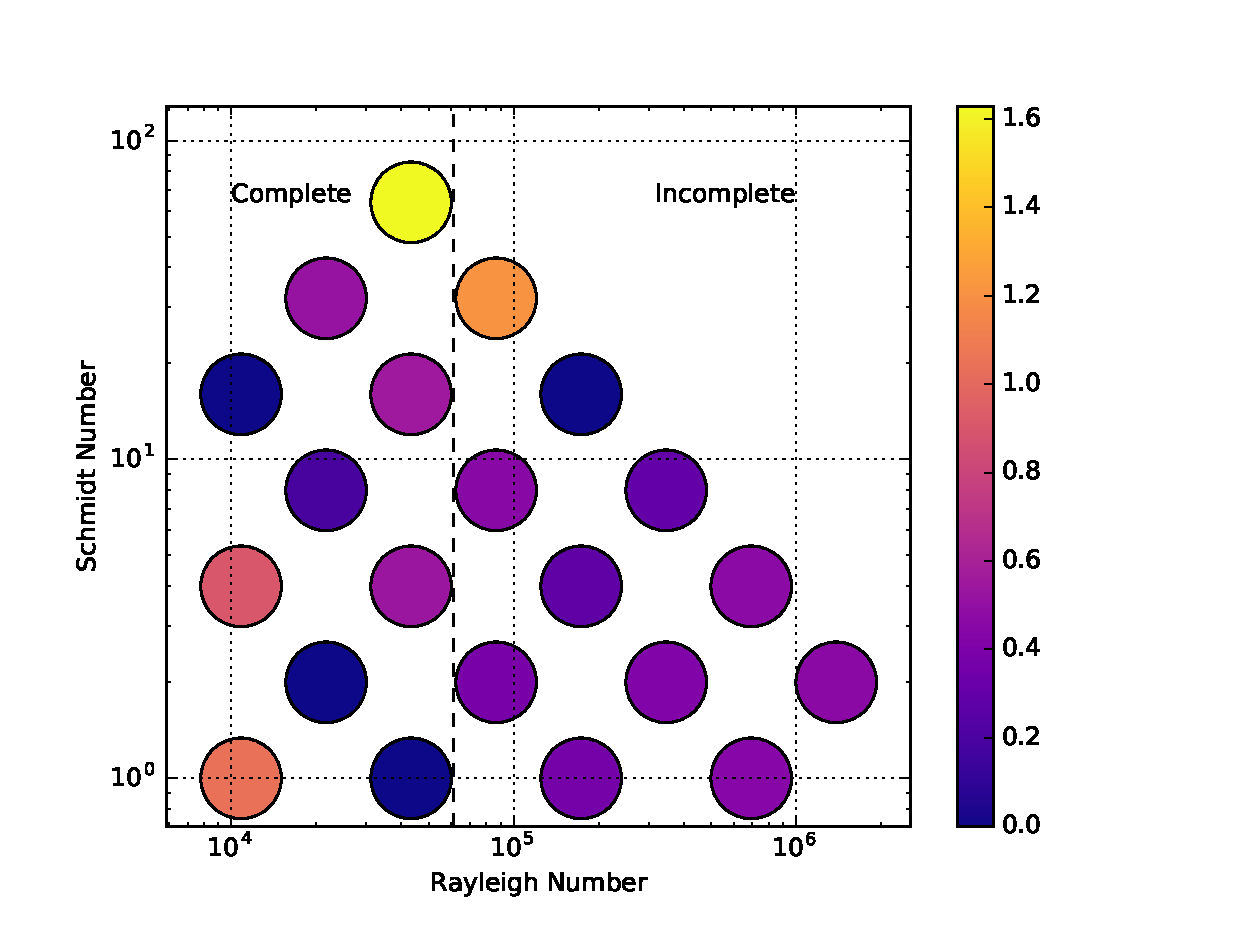
\includegraphics[width=\columnwidth]{figs/C1-vs-Rayleigh-Schmidt}
\caption{ \flabel{C1VsParam}
  Best fit for $C_1$ versus Rayleigh and Schmidt numbers.
  Experiments on the left side of the dashed line completed when the bubble stopped rising.
  Experiments on the right side of the dashed line are incomplete, having approached the vertical boundaries of the simulated domain.
}
\end{figure}

The coefficient $C_1$ is related to the drag coefficient $C_d$ by \eref{prior_c1}.
Therefore we expect it to take a value around or less than $0.64$, which corresponds to the drag coefficient of a flat plate and a surface area $A = \lambda^2$.

The $C_1$ term is most influential early in the flow, so we expect it to be well constrained even in the incomplete trajectories.
However, the $C_1$ term is qualitatively redundant with the $C_3$ inertial term, as they both bound the acceleration but not the velocity.
Similarly, viscous drag is weak but still present at early times.
It is possible that late-time effects that influence $C_2$ could have an indirect effect on the value of $C_1$.

The fit values of $C_1$ are plotted vsersus the Rayleigh and Schmidt numbers in \fref{C1VsParam}.
The majority of trajectories are closely grouped between $0.3$ and $0.6$, which fits the drag coefficient rationale.
However, there are outliers both at $C_1 = 0$ and $C_1 > 0.9$.
These outliers are troubling because each type occurs at both high and low Schmidt number and at low to moderate Rayleigh numbers.
There is no clear pattern, but there are no outliers at the high Rayleigh-number.

\subsubsection{Skin drag coefficient, $C_2$}
\begin{figure}
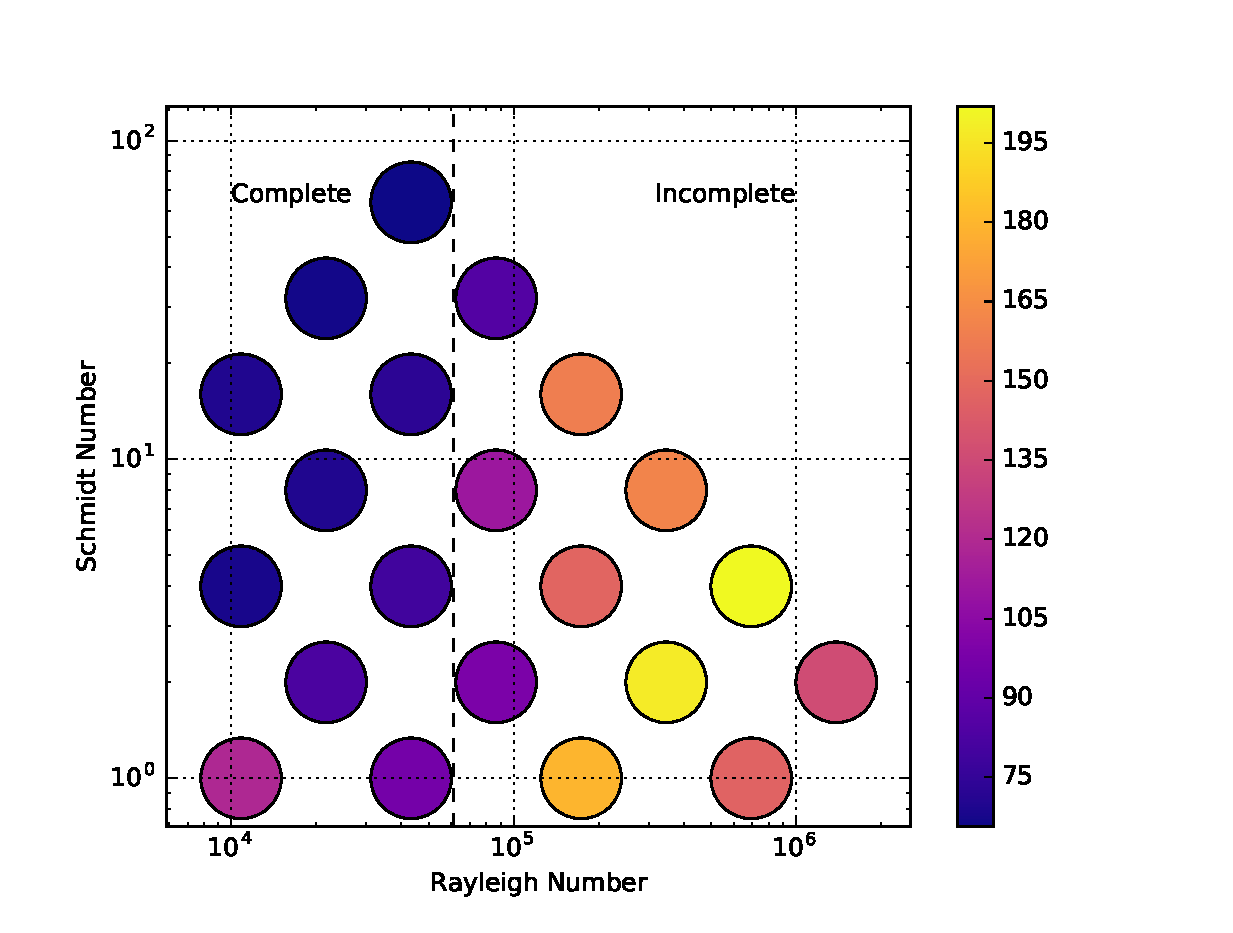
\includegraphics[width=\columnwidth]{figs/C2-vs-Rayleigh-Schmidt}
\caption{ \flabel{C2VsParam}
  Best fit for $C_2$ versus Rayleigh and Schmidt numbers.
  Experiments on the left side of the dashed line completed when the bubble stopped rising.
  Experiments on the right side of the dashed line are incomplete, having approached the vertical boundaries of the simulated domain.
}
\end{figure}

The coefficient $C_2$ scales the viscous drag.
As with $C_1$, $C_2$ can be related to a standard measure of drag, in this case the Darcy friction factor, which provides an estimate of 113.
The $C_2$ term is linear with $h$ and $\dot{h}$, so its influence is greatest at moderate to late times.
Therefore, values of $C_2$ taken from incomplete trajectories should be taken with a grain of salt.

The fit values of $C_2$ are plotted versus the Rayleigh and Schmidt numbers in \fref{C2VsParam}.
For the completed trajectories, $C_2$ is about $60$ and grows slightly with the Grashof number while being nearly independent of the diffusivity.
At higher Rayleigh numbers the incomplete trajectories also show $C_2$ growing with Grashof number, but the effect is much stronger.
There is weaker growth as the diffusivity decreases.
Finally, at the highest Grashof numbers the $C_2$ coefficient moderates again.

The presense of a positive relationship between $C_2$ and the Grashof number in both the complete and incomplete trajectories suggests it is a real effect, though its strength is unclear.
The relationship between $C_2$ and the diffusivity is much weaker and could disappear as the high Rayleigh trajectories are completed.

One possible mechanism for increasing $C_2$ with increasing Grashof number is the development of small amplitude Kelvin-Helmholtz structures on the bubble surface.
These structures are suppressed at low Grashof number and grow more rapidly at higher Grashof number.
They would enhance the transport of momentum across the bubble interface, thereby increasing the viscous drag coefficient.

\subsubsection{Inertial coefficient, $C_3$}
\begin{figure}
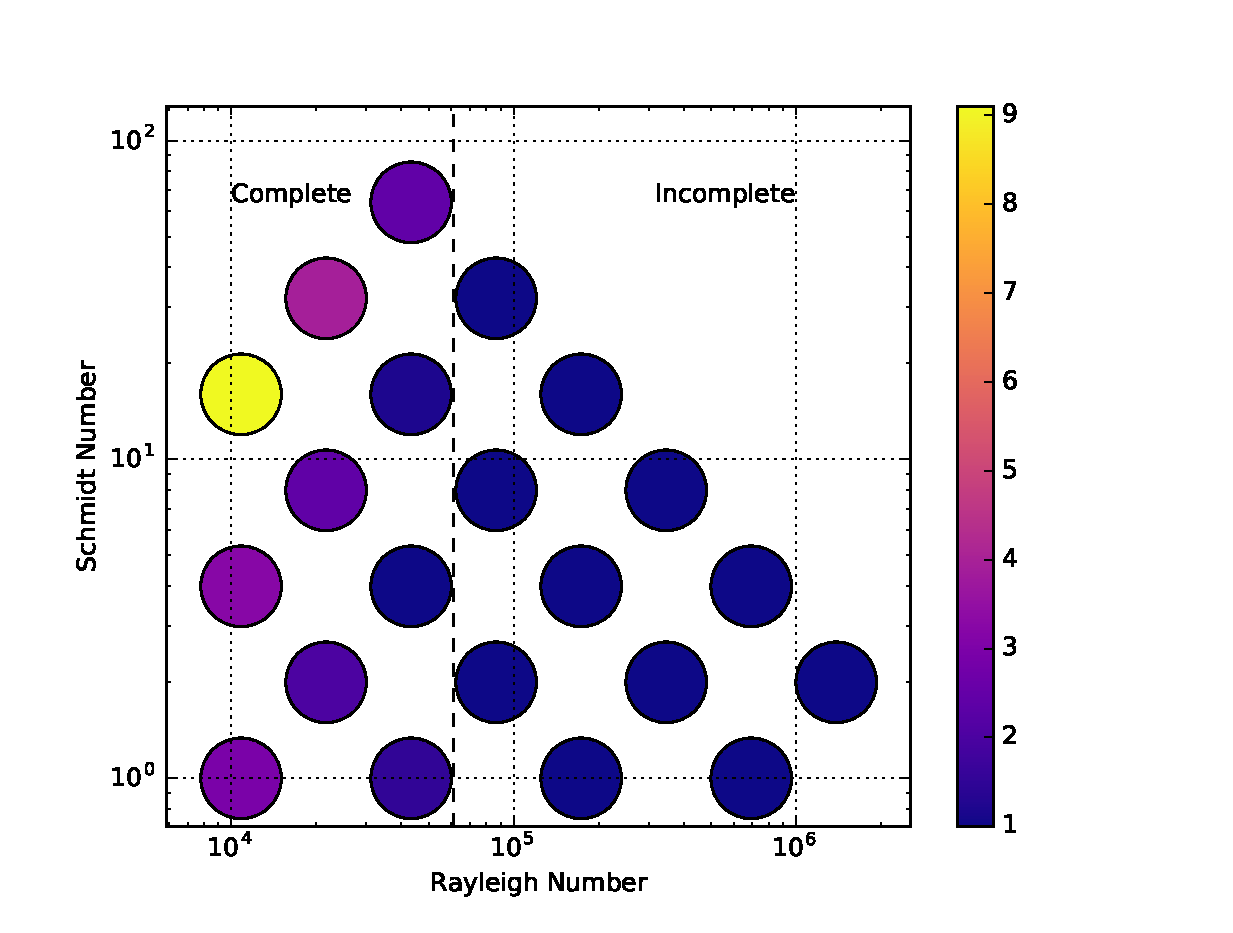
\includegraphics[width=\columnwidth]{figs/C3-vs-Rayleigh-Schmidt}
\caption{ \flabel{C3VsParam}
  Best fit for $C_3$ versus Rayleigh and Schmidt numbers.
  Experiments on the left side of the dashed line completed when the bubble stopped rising.
  Experiments on the right side of the dashed line are incomplete, having approached the vertical boundaries of the simulated domain.
}
\end{figure}

The coefficient $C_3$ gives the ratio of the inertial height to the buoyant height.
For $C_3 = 1$, the maximum bubble acceleration is $A g$ while $C_3 > 1$ represents the entrainment of neutrally or anti-buoyant fluid that contributes to the inertia but not the forcing.
Mixing, which also reduces the ratio of the forcing to the inertia, is accounted for explicitly with the $C_5$ coefficient and fit independently to the mixed volume observable, which prevents it from compensating for entrainment.
The $C_3$ term is linear with the height, so its influence is most pronounced at greater values of the height.

The fit values of $C_3$ are plotted versus the Rayleigh and Schmidt numbers in \fref{C3VsParam}.
The majority of trajectories have $C_3 = 1$, indicating that entrainment is not significant.
For completed low Rayleigh high Schmidt flows $C_3$ increases to a value of $9.1$.
However, the nominal value of $1$ is recovered within the completed trajectories.
Because the $C_3$ term depends on the height, it is relatively underconstrained at lower Rayleigh numbers.
If the model values of $C_4$, $C_6$, or $C_8$ are incorrect, the $C_3$ term has the greatest ability to compensate for the error when the height and velocity are small.
However, the height is still small, so $C_3$ would have to change significantly.
The author belives that $C_3 = 1$ is therefore the nominal value, but there is a breakdown in the model at low Rayleigh numbers that is influencing the fit of $C_3$.
Identifying and correcting this model breakdown would be expected to recover $C_3$ at low Rayleigh number.

\subsubsection{Interfacial area coefficient, $C_5$}
\begin{figure}
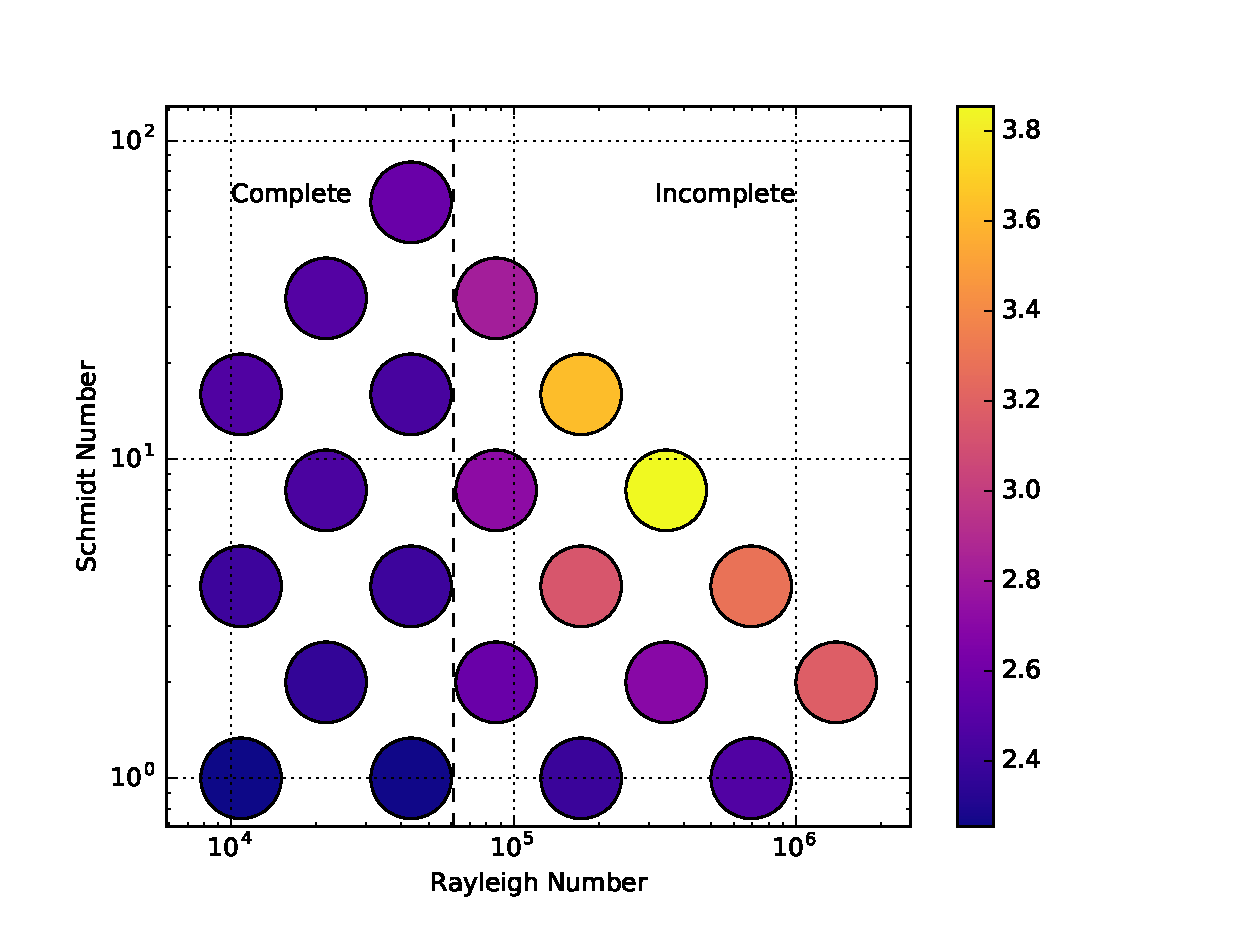
\includegraphics[width=\columnwidth]{figs/C5-vs-Rayleigh-Schmidt}
\caption{ \flabel{C5VsParam}
  Best fit for $C_5$ versus Rayleigh and Schmidt numbers.
  Experiments on the left side of the dashed line completed when the bubble stopped rising.
  Experiments on the right side of the dashed line are incomplete, having approached the vertical boundaries of the simulated domain.
}
\end{figure}

The parameter $C_5$ gives the ratio of the span-wise circumference of the scalar interface to the wavelength.
If the bubble were rectangular in cross section with diameter $\lambda / 2$, then $C_5 = 4$.
If the bubble had a circular cross section with diameter $\lambda / 2$, then $C_5 \approx \pi$.
If the bubble diameter is less than a half-wavelength, then $C_5 < \pi$.
The mixing width $\delta$ increases with time, so the $C_5$ term is most influential at late times.
Therefore, the values of $C_5$ in the incomplete trajectories should be taken with a grain of salt.

The fit values of $C_5$ are plotted versus the Rayleigh and Schmidt numbers in \fref{C5VsParam}.
Among the completed trajectories, $C_5$ is a much stronger function of the Schmidt number than the Rayleigh number, increasing in both.
The values are between 2 and 3, indicate a thinning of the bubble that decreases the mix rate by reducing surface area and total quantity of pure light fluid transported into the dense fluid.

The incomplete trajectories contain richer behavior, with a local maximum at $\text{Ra} = 10^{5.5}$ and $\text{Sc} = 8$.
In aggreate, higher Rayleigh number trajectories have increasing $C_5$ with decreasing diffusivity.
The dependence on the Grashof number is peaked at $\text{Gr} \approx 4.3 \times 10^4$.
The increasing $C_5$ with increasing Schmidt number in the completed trajectories is consistent with these two effects, which can be seen the smoothness of \fref{C5VsParam}.

A possible mechanism for increasing $C_5$ with decreasing diffusivity is the development of structures on the scalar interface the increase the effective surface area.
This is related to the Kelvin-Helmholtz structures proposed to explain increasing $C_2$ with Grashof number, but with additional dependence on the diffusivity which can otherwise smear out the structures.

Another possible mechanism is a change in the bubble diameter.
Higher Grashof number bubbles have thinner momentum boundaries, allowing more buoyant fluid to flow freely through the stem of the bubble.
This sustains the bubble diameter at late times, while more viscous bubbles can thin.
This would explain an increase of $C_5$ with the Grashof number.

The authors have no mechanism by which to explain the local maximum value, so we expect it to disappear with trajectory completion by default.
It would be very interesting if it remained, and further motivates completing the high Rayleigh number trajectories.

\subsubsection{Pure fluid coefficient, $C_7$}
\begin{figure}
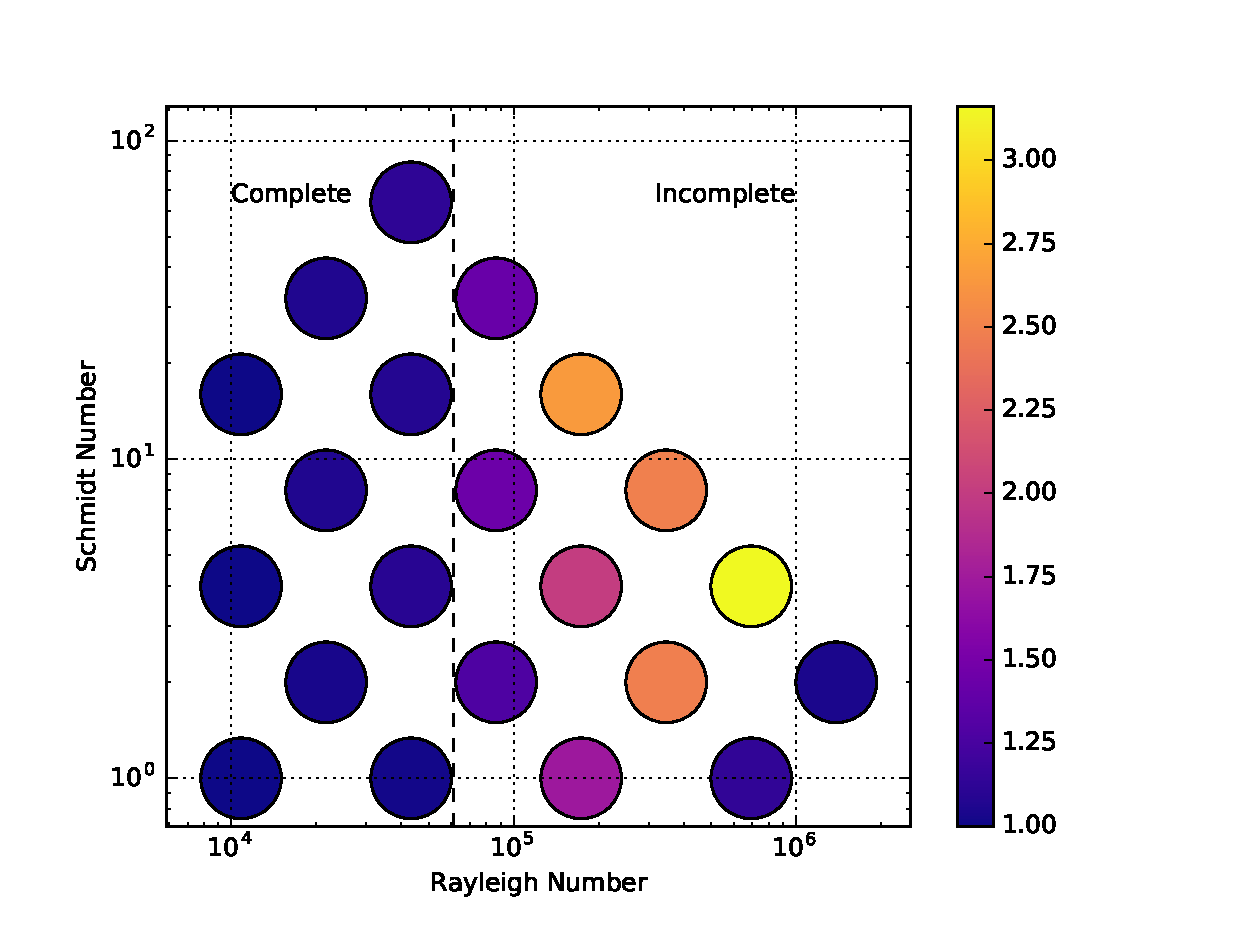
\includegraphics[width=\columnwidth]{figs/C7-vs-Rayleigh-Schmidt}
\caption{ \flabel{C7VsParam}
  Best fit for $C_7$ versus Rayleigh and Schmidt numbers.
  Experiments on the left side of the dashed line completed when the bubble stopped rising.
  Experiments on the right side of the dashed line are incomplete, having approached the vertical boundaries of the simulated domain.
}
\end{figure}

Similar to $C_3$, $C_7$ gives the ratio of the buoyant volume to the maximal mixed volume.
A value of $C_7 = 1$ implies the effective Atwood number is zeroed when $M(t) = \lambda^2 h$.
Values greater than one imply that some portion of the positively buoyant fluid that would be in bubble has become entrained into the neighboring spike, allowing $M(t) > \lambda^2 h$ while retaining net buoyancy.

The fit values of $C_7$ are plotted versus the Rayleigh and Schmidt numbers in \fref{C7VsParam}.
The complete trajectories all have $C_7 \approx 1$, while the incomplete trajectories at higher Rayleigh numbers have increasing $C_7$.
It is possible that at higher Rayleigh numbers some volume of light fluid detaches from the bubble and is transported into the spike.
However, it is more likely that in the incomplete cases $C_7$, which influences the dynamics most at high mixing volumes, is underconstrained.
In that case, we would expect $C_7 \approx 1$ with no dependence on the Grashof, Rayleigh, or Schmidt numbers when the trajectories are completed.

